\documentclass[12pt]{article}
\usepackage{geometry} % see geometry.pdf on how to lay out the page. Theres lots.
\geometry{a4paper} % or letter or a5paper or ... etc
% \geometry{landscape} % rotated page geometry

\usepackage{graphicx}
\usepackage[english]{babel}
\usepackage{enumitem}%can be used for automatic numbering of requirements.
\usepackage{paralist}

\newlength{\testlabellength}
\settowidth{\testlabellength}{Test 100.10.10}

\date{} % delete this line to display the current date

% Begin document.
\begin{document}

\setlength{\parindent}{0em}
%==================================
% F�rs�ttsblad. 
\begin{titlepage}

\begin{minipage}{0.5\textwidth}
\begin{flushleft} % Responsible persons, write on separate lines
\textit{Lund University\\ ETS170: Requirements Engineering}\\
\end{flushleft}
\end{minipage}
~
\begin{minipage}{0.4\textwidth}
\begin{flushright}
\today

\end{flushright}
\end{minipage}\\[3cm]

	\centering
	{\scshape\LARGE ShopMate \par}
	\vspace{0.5cm}
	\rule{1\textwidth}{.6pt} \par
	{\huge\bfseries Requirements Specification\par}
	\rule{1\textwidth}{.6pt} \par
	\vspace{2cm}
%	{\Large\itshape }

%==================================
% The authors down to the left. 
\vfill
\begin{flushleft}
	\textit{By Group I:}\\
	Daniel Dornl\"{o}v\par 
	David Cartbo\par
	Jonathan Lundholm\par 
	Kristoffer Hilmersson\par
	Marcus Hilliges\par 
	Thomas Strahl\par
	\end{flushleft}
\end{titlepage}

\newpage
\begin{center}

%==================================
% The version history of this document. 
\textit{\large Version History}

    \begin{tabular}{ | l | l | l | p{5cm} |}
    \hline
    \textbf{Version}	& \textbf{Date}		& \textbf{Description}			\\ \hline
    0.1			& 2015-11-22 			& First release			\\ \hline
   	0.2			& 2015-12-7			& Release 2 			\\ \hline
    \end{tabular}
\end{center}

%==================================
% Introduction
\section*{Introduction}
This document describes the functional, data, quality and design requirements for an iOS and Android based application that 
communicates with a server and Smart-Watches. The product aims to assist the user in navigating the mall and to the users parked car, 
get an overview of the layout of the mall,  keep track of what errands the user has in the mall and display offers from stores in the mall. 

%==================================
% Business Goals
\subsection*{Business Goals}

The purpose of the product is the enhance the quality of a customer visit by offering some features that facilitates the stay. 
With the provided functionality of the product, the customer satisfaction will increase, as well as the number of visiting customer and the 
number of sales the stores. This will enable the mall owner to charge the stores higher rents and a higher revenue for the stores in the mall.

%==================================
% Business Goals

\subsection*{Terminology}
	\begin{description}
	\setlength{\itemsep}{0pt}
	\item[The app] is referring to the ordered application for a shopping mall, i.e. the ordered product.
	\item[The user] is referring to the person using the application on their device.
	\item[Device] is referring to the unit the user is running the app on, e.g. mobile phone and smart-watch.
	\item [Offers] are store-products or services that are being sold att a lower price in the stores a the mall. Offers are displayed on the users screen of their devices.
	\item [The server/database] is where all data about stores, offers, store-products, maps and so on are stored.
	\item [Store] refers to companies located in the mall. 
	\item [Store-Product] refers to items/products being sold in the stores, not the product that is being developed.
	\item [Location] refers to the location of a user or a store in the shopping mall. 
	\item [Shopping list] refers to a list with items or store-products that the user has added to a list and intends to buy while at the mall.
\end{description}

\subsection*{Context Diagram}
ShopMate has an excessive inner domain, communicating with various other systems. In order to fulfill some of the fundamental requirements, this is necessary. Figur 1 below represents the domain level of ShopMate, displaying the systems needed to provide the desired functionality. 

\begin{figure}[h]
    \centering
    \includegraphics[width=0.9\textwidth]{../images/Context_Diagram.png}
    \caption{A context diagram describing the domain level of ShopMate. }
    \label{fig:contdiag}
\end{figure}

%==================================
% This is where the requirements start.
%==================================

\section*{Requirement Specification}

%==================================
% Goal Level. 
\subsection*{Goal Level}
The goal level requirements comprises of goals for both the customers and the owners of the shopping mall. \\

\underline{Business --- Customer satisfaction} \\ The product shall increase the shopping malls customer satisfaction.\\ \par

\underline{Business --- Mall revenue} \\ The product shall increase the malls revenue by 4�\%.\\ \par

\underline{Business --- More customers} \\ The product shall help increase the number of visiting customers to the mall by 8 \%.\\ \par

\underline{Business --- Increased sales} \\ The product shall help increase the number of sales the stores have by 3 \%. \\ \par

\underline{Business --- Impulse sales} \\ The product shall increase the number of impulse buys of store-products by 10 \%.

%==================================
% Requirements on Domain Level. 
\subsection*{Domain Level}

The domain level concerns the surroundings of the system and how the system interacts with it. \\

 \underline{Data --- Attributes} \\ The product shall store data according to figure \ref{fig:er} and figure \ref{fig:user}.  \\ \par

 \underline{Data --- Product} \\ The product shall have data provided by the stores on stock balance, prices and offers on store-products provided by the stores.\\ \par
 
 \underline{Data --- Registration} \\ The product shall support registration of store offers from different stores as shown in figure \ref{fig:store} and 
 be able to show products like figure \ref{fig:product}. \\ \par

\underline{Navigation --- Find location} \\ The product shall be able to assist the user to get from its current location to a specified location by the user in the mall. e.g. a store, toilet, elevator and so on. \\ \par

\underline{Misc --- No connection} \\ The product shall work without being connected to the internet, to limit data traffic. Without internet connection the product will help the user navigate in the mall and navigate to their parked car. \\�\par

\underline{Navigation --- Public information} \\ The product shall provide public information, such as location of handicap toilets, elevators, ATM machines, etc. With this information the user shall be able to navigate to the correct position in the mall.




\subsubsection*{Parking}

\underline{Parking --- Register parked car} \\ The user shall be able to register the location of the parked vehicle. \\ \par 

\underline{Parking --- Guide to parked car} \\ The product shall be able to guide the user to their parked vehicle. 


%==================================
% Requirements on Product Level. 
\subsection*{Product Level}



\subsubsection*{Smart-Watch}

\underline{Smart-watch --- General} \\ The product shall support connecting a smart-watch to it. To help the user navigate and get offers from stores without having to interact with their smartphone. \\ \par 

\underline{Smart-watch --- Navigation} \\ The product shall support navigation on the Smart-Watch screen. \\ \par 

\underline{Smart-watch --- Guide to parked car} \\ The product shall support helping the user find where they parked their car. \\ \par 

\underline{Smart-watch --- Offers} \\ The product shall support the functionality to store offers in a smart-watch. \\ \par 

\underline{Smart-watch --- Shopping list} \\ The product shall be able to display the users shopping-list on the Smart-Watch. \\ \par 

\underline{Smart-watch --- Not required} \\ The product shall work without a Smart-Watch. Not all customers have smart-watches and it can therefore not be a requirement to use the product with one.



\subsubsection*{Additional Functionality}

\underline{Transportation --- Public transport} \\ The product shall support information about departures using public transportation. \\ \par 

\underline{Misc --- Create shopping list} \\ The user shall be able to create a shopping list. The store-products shall be searched for by 
type and display what store has that type of store-product so the user can select what store and store-product he or she wants to add to the shopping list. \\ \par 

\underline{Misc --- Rating system} \\ The product shall have a rating system for stores in the mall that users can use to rate stores. \\�\par

\underline{Misc --- Platforms} \\ The product shall be implemented for Android devices and iOS devices.\\ \par 

\underline{Data --- Database contents} \\ The database shall contain the store-products sold in the shopping mall, and provide information which store that sells them.




\subsubsection*{Navigation}

\underline{Navigation --- Find user in mall} \\ The product shall have a function for locating the user in the shopping mall. This function will help the user to know what floor he or she is on, and where on that floor the user is currently located. \\ \par

 \underline{Navigation --- Find location 2} \\ The product shall have a function for directing the user to a specific location in the mall.
 
 
 
\subsubsection*{Offers}
 
\underline{Offer --- Location offers} \\ The product shall display a new offer if the user is within 10 meters to a store. Offers shall be relevant to the users location in the mall. \\ \par
 
\underline{Offer --- Display specific offers} \\ The product shall display specific offers designed by the stores if the user enters their stores. \\ \par
 
\underline{Offer --- Limit of displaying offers} \\ The product may show a new offer every 120 seconds.

\subsubsection*{Parking}
 
 \underline{Parking --- Register parked car 2} \\ The product shall provide a function to register where the users vehicle is parked. \\�\par
 
 \underline{Parking --- Guide to parked car 2} \\ The product shall provide a function to locate the users parked vehicle. \\�\par
 
 \underline{Parking --- Find free parking place} \\ The product shall have the function for displaying what parking places are free and assist the user to locate the free parking places.
 

 \subsubsection*{Quality Requirements}
 
 
 \underline{Navigation --- Precision of positioning} \\ The product positioning shall have a resolution no greater than 5 m. \\�\par
 
 \underline{Misc --- Server up-time} \\ The server shall have at least 99 \% up-time over a year of runtime. \\�\par
 
  \underline{Misc --- Accuracy locate car} \\ The product shall locate the users parked car with an accuracy of at least 5m. When the user uses the function "navigate to parked car". \\�\par
  
  \underline{Misc --- Locate user speed }\\ The product shall locate the users location with in 3 seconds after staring the application 90 \% of the time.


%==================================
% Requirements on Design Level. 
\subsection*{Design Level}

 
 \underline{GUI --- Navigation screen} \\ The product shall provide the screen shown in figure \ref{fig:nav} to help the user navigate.\\�\par

 \underline{Data --- General store information} \\ The product shall have a database to store general information about the stores. \\�\par
 
 \underline{GUI --- Understandable interface} \\ The product shall be easy to understand, a novice user shall be able to navigate the interface after the first time the product has been used. \\�\par

 \underline{Offer --- Non-annoying commercials} \\ The product shall not be annoying to use or clutter the screen with offers. In other words offers 
 that are displayed on the screen shall not cover the whole screen they could look like displayed in figure \ref{fig:offer}.  \\�\par
 
  \underline{Misc --- Fast server connection} \\ The product shall connect to the server with in 5 seconds after starting the product  95 \% of 
  the time, so the server and the user device is updated with the latest offers and potential new stores. This shall not hinder the application from working. 
  This shall be done in the background. \\�\par
  
   \underline{Smart-Watch --- Screen appearance} \\ The Smart-Watch screen appearance shall look as in figure \ref{fig:smartwatch}.
   
\subsubsection*{Offers}
 
\underline{GUI --- Non covering offers} \\ The product shall display offers from stores without covering the user device screen.
 
 \newpage
 \section*{Appendix A} \label{app:appA}
Appendix A holds the figures referred to in the requirements.
 
 
 \begin{figure}[h]
    \centering
    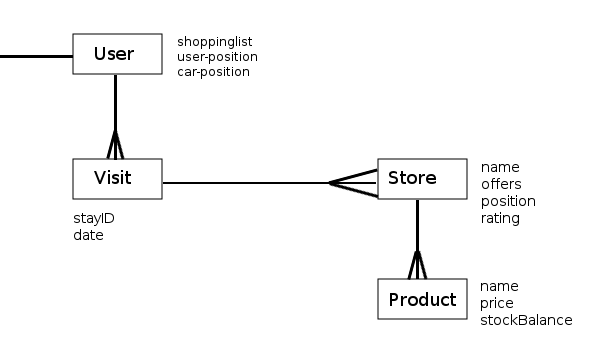
\includegraphics[width=0.7\textwidth]{../images/erdiags.png}
    \caption{Refers to the requirement "Data --- Attributes".}
    \label{fig:er}
\end{figure}

\begin{figure}[h]
    \centering
    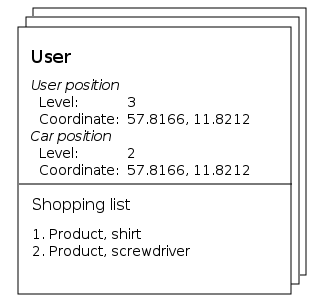
\includegraphics[width=0.4\textwidth]{../images/vw_user.png}
    \caption{Refers to the requirement "Data --- Attributes."}
    \label{fig:user}
\end{figure}

\begin{figure}[h]
    \centering
    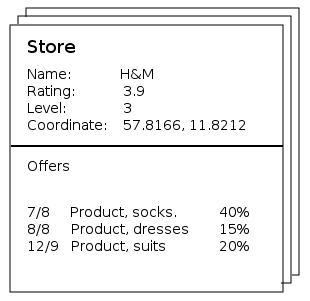
\includegraphics[width=0.4\textwidth]{../images/vw_store.png}
    \caption{Refers to the requirement "Data --- Registration."}
    \label{fig:store}
\end{figure}

\begin{figure}[h]
    \centering
    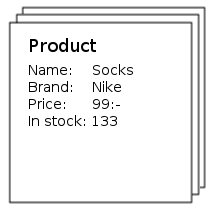
\includegraphics[width=0.35\textwidth]{../images/vw_product.png}
    \caption{Refers to the requirement "Data --- Registration."}
    \label{fig:product}
\end{figure}
 
  \begin{figure}[h]
    \centering
    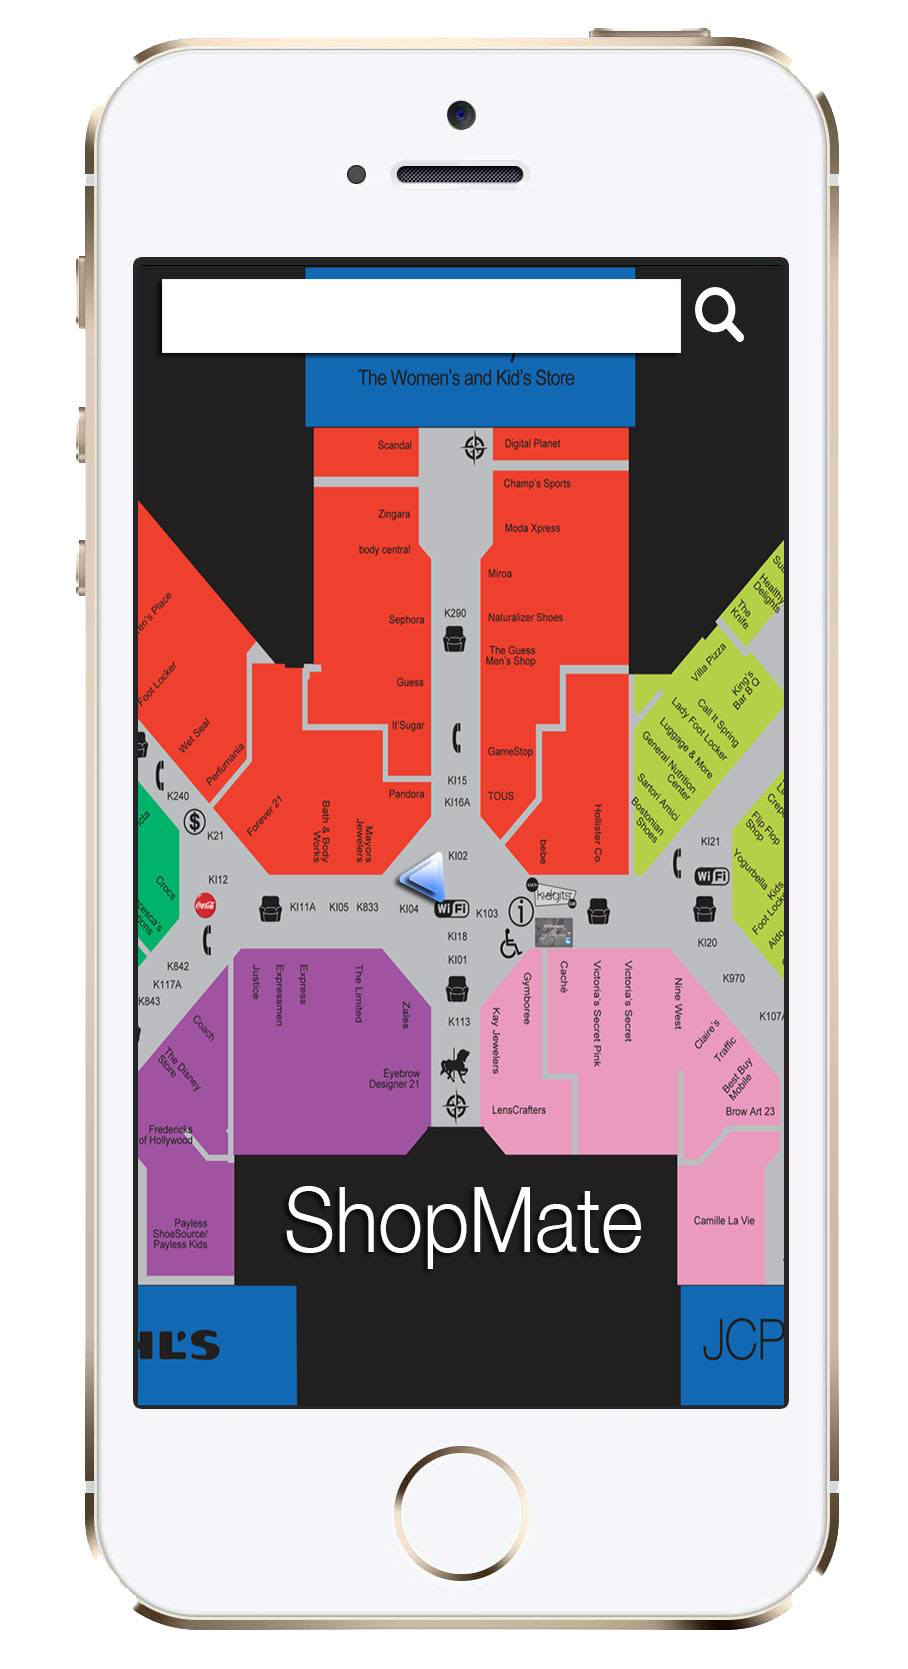
\includegraphics[width=0.3\textwidth]{../images/nav.png}
    \caption{Refers to the requirement "GUI --- Navigation screen".}
    \label{fig:nav}
\end{figure}

  \begin{figure}[h]
    \centering
    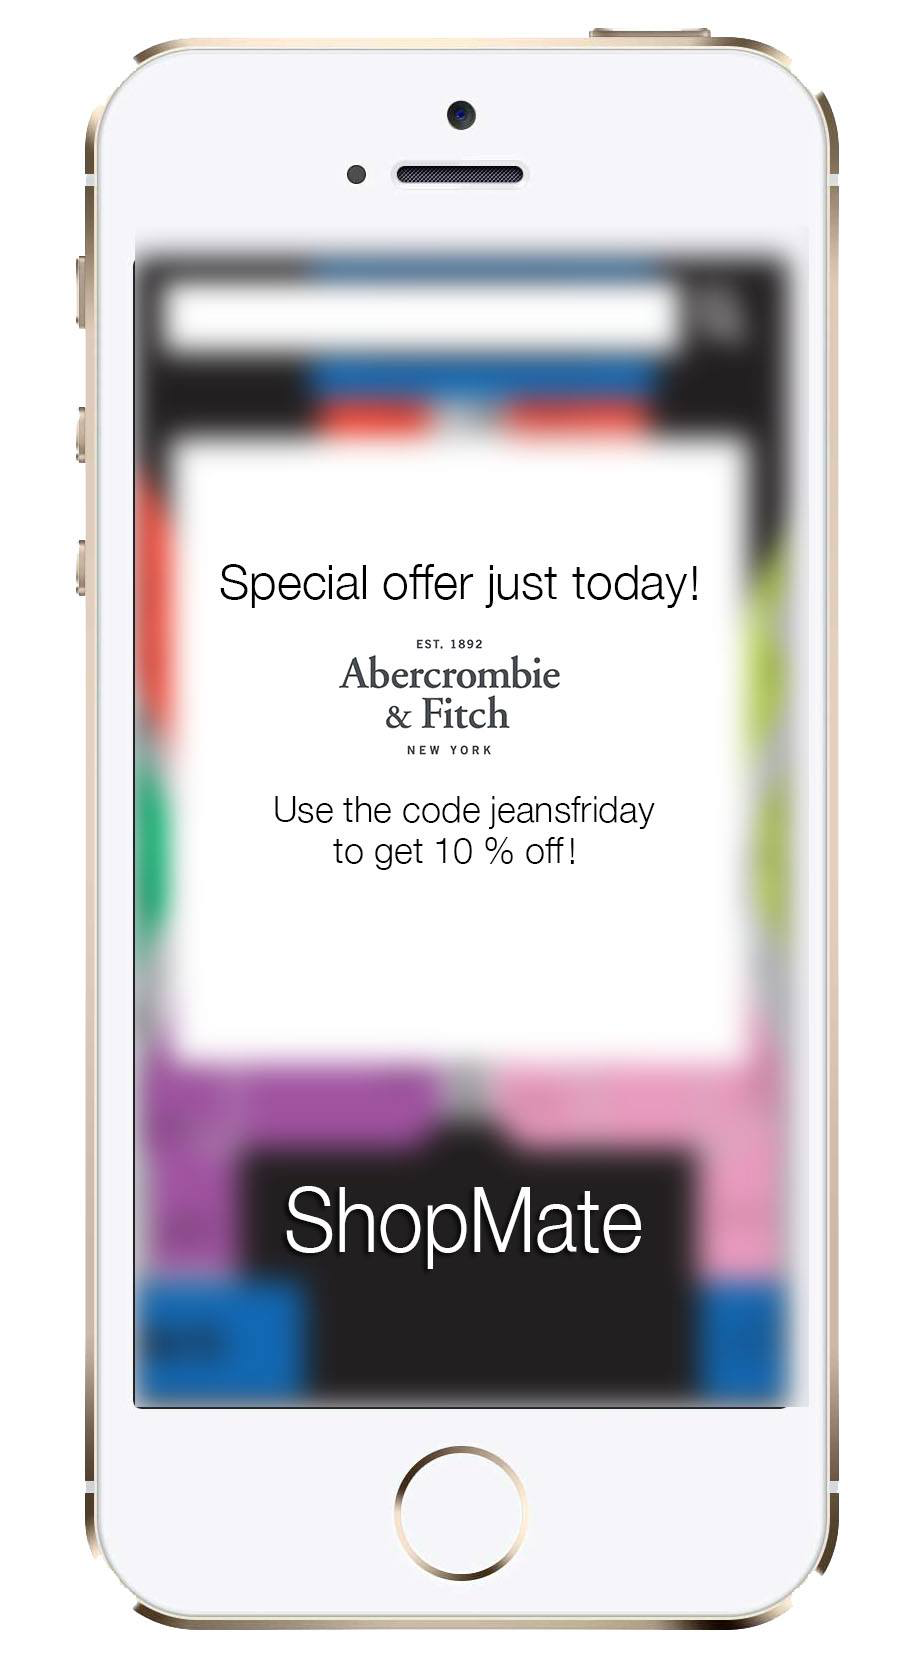
\includegraphics[width=0.3\textwidth]{../images/offer.png}
    \caption{Refers to the requirement "Offer --- Non-annoying commercials".}
    \label{fig:offer}
\end{figure}


  \begin{figure}[h]
    \centering
    \includegraphics[width=0.5\textwidth]{../images/smartwatches.png}
    \caption{Refers to the requirement "Smart-Watch --- Screen appearance".}
    \label{fig:smartwatch}
\end{figure}

\end{document}